% Provenance (never printed): see sources/outline_sources.md (Year 3:
% Darcy's law; permeability; aquifer types; the groundwater-flow equation;
% pumping tests; solute transport, in principle).
% Brief: sources/book5/BRIEFS.md, ch. 23. Curves from figdata/bachelor-3/
% theis.py, flow_net.py and advection_dispersion.py; the site of Varden-3 from
% figdata/shared/region.py (read only). Exercise and problem values in the
% Book 5 scratch calculator calc/ch23.py. The wells, the dam, the tests and
% the solutes are invented.
\chapter{Hydrogeology}\label{ch:b3:hydrogeology}

A new well pumps \qty{2160}{m^3} of water a day from a limestone a few
hundred metres below a farm. Nothing happens to the farm's own well at
first. A month later its water stands nearly \qty{2}{m} lower, although it is
a kilometre away and the pumping station has never drawn a drop from it. The
water level round the new well has not fallen uniformly: it has sunk into a
cone, and the cone has grown, quickly, through a rock in which the water
itself moves a few centimetres a day. This chapter builds the physics that
predicts both numbers, the fast spread of the pressure and the slow travel
of the water, from one empirical law found in 1856.
% ledger: heath:darcy

\begin{recall}
Porosity, permeability, the water table, groundwater, aquifers, springs
and wells are in the school books, with the residence time of water and
fossil groundwater. Viscosity, Poiseuille's law for the flow in a tube
and the diffusion equation are in the physics books. The error function
and the solutions of the diffusion equation that use it are in
Chapter~\ref{ch:b3:lithosphere-thermal-models}. The Varden Hills, the
series' invented region, with its sandstone, limestone, shale and chalk,
are the region of the exercises since the school books.
\end{recall}

\section{Head and Darcy's law}\label{sec:b3:hydrogeology:darcy}

Water underground moves from where its mechanical energy per unit weight is
high to where it is low. Because it moves slowly, its kinetic energy is
negligible, and that energy has two parts: the height of the water and its
pressure.

\begin{definition}[Hydraulic head; hydraulic gradient]\label{def:b3:hydrogeology:head}
The \emph{hydraulic head}\index{hydraulic head} at a point of the
saturated ground is
\[
h = z + \frac{p}{\rho g} ,
\]
the sum of the \emph{elevation head} $z$ of the point above a datum and the
\emph{pressure head} $p/(\rho g)$, $p$ being the pressure of the water above
the atmospheric pressure. It is the elevation to which water rises in a
tube, a piezometer, open only at that point. The \emph{hydraulic
gradient}\index{hydraulic gradient} is $\nabla h$; its size between two
points a distance $L$ apart along the flow is $\Delta h/L$.
\end{definition}

\begin{omfigure}
\centering
\begin{tikzpicture}[>=stealth, font=\small, x=1cm, y=1cm]
\fill[omLithAlluv!60] (0,-0.6) rectangle (7,3.2);
\fill[omSea!45] (0,-0.6) rectangle (7,1.9);
\draw[thick, brown!60!black] (0,3.2) -- (7,3.2);
\draw[omDef, dashed] (0,1.9) -- (7,1.9);
\node[omDef, font=\scriptsize, anchor=south east] at (6.9,1.92) {water table};
% piezometer
\fill[white] (3.3,0.4) rectangle (3.7,4.0);
\draw[thick] (3.3,0.7) -- (3.3,4.0); \draw[thick] (3.7,0.7) -- (3.7,4.0);
\draw[thick, densely dotted] (3.3,0.4) -- (3.3,0.7); \draw[thick, densely dotted] (3.7,0.4) -- (3.7,0.7);
\fill[omSea!70] (3.32,0.4) rectangle (3.68,2.6);
\draw[omDef, thick] (3.3,2.6) -- (3.7,2.6);
\fill (3.5,0.55) circle (0.06);
\node[font=\scriptsize, anchor=west] at (3.75,0.55) {screen, at the point $P$};
% datum
\draw[black!60] (0,-0.6) -- (7,-0.6);
\node[font=\scriptsize, anchor=north west] at (0,-0.62) {datum, $z = 0$};
% heads, on the left of the tube
\draw[<->] (2.5,-0.6) -- node[left, font=\scriptsize] {$z$} (2.5,0.55);
\draw[<->] (2.5,0.55) -- node[left, font=\scriptsize] {$p/\rho g$} (2.5,2.6);
\draw[black!40, densely dashed] (2.4,0.55) -- (3.3,0.55);
\draw[black!40, densely dashed] (1.0,2.6) -- (3.3,2.6);
\draw[<->, thick, omThm] (1.1,-0.6) -- node[left, font=\scriptsize] {$h$} (1.1,2.6);
\node[font=\scriptsize, anchor=south] at (3.5,4.0) {piezometer};
\end{tikzpicture}

\par\smallskip{\small A piezometer, a tube open only at its screen. The
water stands in it at the \omterm{def:b3:hydrogeology:head}{hydraulic head} of the point $P$: its elevation
$z$ plus its pressure head. Here the level in the tube is above the water
table, as it is where the water rises towards a spring or a
river.}\label{fig:b3:hydrogeology:head}
\end{omfigure}

In 1856 Henry Darcy, a French engineer, measured the flow of water through
columns of sand and found it proportional to the loss of head per unit
length. The flow is laminar: the water follows separate streamlines.
% ledger: heath:darcy

\begin{theorem}[Darcy's law]\label{thm:b3:hydrogeology:darcy}
In a saturated porous medium the volume of water crossing unit area per
unit time is
\[
\vec q = -K\,\nabla h ,
\]
where $K$ depends on the medium and on the fluid. In a medium whose pores
are parallel straight tubes of radius $a$ occupying a fraction $n$ of the
volume, Poiseuille's law gives this law with
\[
K = \frac{k\rho g}{\mu}, \qquad k = \frac{na^2}{8} ,
\]
$\mu$ being the viscosity of the water.
\end{theorem}
\index{Darcy's law}

\begin{proof}
The first statement is Darcy's empirical law. In a tube of radius $a$
along the flow, Poiseuille's law gives the mean velocity $\bar u =
-(a^2/8\mu)\,\mathrm d(p + \rho gz)/\mathrm dl = -(a^2\rho g/8\mu)\,\mathrm
dh/\mathrm dl$, since $p + \rho gz = \rho g h$. The tubes occupy the
fraction $n$ of any cross-section, so the volume per unit total area is
$q = n\bar u = -(na^2/8)(\rho g/\mu)\,\mathrm dh/\mathrm dl$.
\end{proof}

Real pores are not straight tubes; the theorem shows the form of the law
and how it scales. The flow is proportional to the gradient, to the square
of the size of the pores, and inversely to the viscosity: the same sand
lets water through faster when it is warm.

\begin{definition}[Specific discharge; hydraulic conductivity; intrinsic permeability]\label{def:b3:hydrogeology:darcy}
The \emph{specific discharge}\index{specific discharge} $\vec q$ is the
volume of water crossing unit area of the medium, grains and pores
together, per unit time. The \emph{hydraulic
conductivity}\index{hydraulic conductivity} $K$ is the coefficient of
\omterm{thm:b3:hydrogeology:darcy}{Darcy's law}, in \unit{m/s} or \unit{m/d}. The \emph{intrinsic
permeability}\index{intrinsic permeability} of the medium is $k =
K\mu/(\rho g)$, in \unit{m^2}: it depends on the medium alone.
\end{definition}

The \omterm{def:b3:hydrogeology:darcy}{hydraulic conductivity} of the rocks ranges through twelve orders of
magnitude, as few physical quantities do. Read off the chart of a classic
survey of the subject, typical ranges, in metres per day, are: clay
\num{e-7} to \num{e-4}; silt and loess \num{e-3} to 2; silty sand 0.04 to
10; clean sand 0.3 to 150; gravel 100 to 4000; shale \num{e-8} to
\num{e-4}; sandstone \num{e-5} to 0.4; carbonate rocks \num{e-4} when they
are only fractured to several thousand when they are cavernous; igneous and
metamorphic rocks below \num{e-8} when unfractured to a few when
fractured. Most rocks also conduct water better along their bedding than
across it.
% ledger: heath:darcy, heath:k-chart

The \omterm{def:b3:hydrogeology:darcy}{specific discharge} is a flux through the whole area; the water flows
only through the pores, and faster.

\begin{definition}[Seepage velocity]\label{def:b3:hydrogeology:seepage}
The \emph{seepage velocity}\index{seepage velocity} is $\vec v = \vec
q/n_e$, the mean velocity of the water in the pores, $n_e$ being the
effective porosity, that of the connected pores through which the water
flows.
\end{definition}

A coarse sand with $K = \qty{60}{m/d}$, a gradient of 1 in 1000 and a
porosity of 0.20 moves its water at \qty{0.3}{m/d}; a clay with $K =
\qty{e-4}{m/d}$, a gradient of 1 in 10 and a porosity of 0.50, at
\qty{2e-5}{m/d}, less than a centimetre a year. Groundwater does not flow
in underground rivers, except in the caves of limestones and the tubes of
lavas. These are averages: where a pollutant travels, its fastest part may
go several times faster.
% ledger: heath:velocity

\section{Aquifers}\label{sec:b3:hydrogeology:aquifers}

\begin{definition}[Confined and unconfined aquifers; aquitard]\label{def:b3:hydrogeology:aquifer-types}
An \emph{unconfined aquifer}\index{unconfined aquifer} is an aquifer whose
upper surface is the water table. A \emph{confined
aquifer}\index{confined aquifer} is an aquifer overlain by a layer of much
lower conductivity, so that the water in it is under pressure: in a well
that reaches it, the water rises above the top of the aquifer, to its
potentiometric surface. A layer of low conductivity that slows but does not
stop the passage of water between aquifers is an
\emph{aquitard}\index{aquitard}.
\end{definition}

\begin{definition}[Transmissivity; storativity; specific yield]\label{def:b3:hydrogeology:storage}
The \emph{transmissivity}\index{transmissivity} of an aquifer of thickness
$b$ is $T = Kb$, the flow per unit width under unit gradient, in
\unit{m^2/d}. Its \emph{storativity}\index{storativity} (or storage
coefficient) $S$ is the volume of water released per unit area of the
aquifer when the head falls by one unit; it is dimensionless. The
\emph{specific yield}\index{specific yield} $S_y$ of a rock is the volume
of water that drains from it by gravity per unit volume when the water
table falls through it.
\end{definition}

The two kinds of aquifer release water in different ways. In a \omterm{def:b3:hydrogeology:aquifer-types}{confined
aquifer} the head falls but the pores stay full: the water expands a
little, and the aquifer, carrying more of the weight of the rocks above,
is compressed a little. The expansion of the water alone releases about
\num{9e-7} cubic metre per cubic metre of aquifer and per metre of head;
with the compression, the \omterm{def:b3:hydrogeology:storage}{storativity} of most \omterm{def:b3:hydrogeology:aquifer-types}{confined aquifers} is
\num{e-5} to \num{e-3}. In an \omterm{def:b3:hydrogeology:aquifer-types}{unconfined aquifer} the water table falls and
the pores above it drain: the \omterm{def:b3:hydrogeology:storage}{storativity} is the \omterm{def:b3:hydrogeology:storage}{specific yield}, about 0.1
to 0.3, a hundred to ten thousand times larger. The transmissivities of
the aquifers in use range from less than \qty{1}{m^2/d} in fractured rocks
to \qty{100000}{m^2/d} in cavernous limestones and lava flows. Where the
head of a \omterm{def:b3:hydrogeology:aquifer-types}{confined aquifer} is drawn down for a long time, the clays in and
around it drain and compact, and the ground above subsides.
% ledger: heath:storage, heath:transmissivity

\begin{omfigure}
\centering
\begin{tikzpicture}[>=stealth, font=\small, x=1cm, y=1.1cm]
\begin{scope}
\clip (0,-1.3) -- (0,2.0) -- (3.5,2.9) -- (5,3.5) -- (7.5,4.2) -- (11,3.8) -- (11,-1.3) -- cycle;
\fill[lith sandstone] (0,-1.3) rectangle (11,4.5);
\fill[lith limestone] (0,1.8) -- (11,-0.95) -- (11,0.05) -- (0,2.8) -- cycle;
\fill[lith shale] (0,2.8) -- (11,0.05) -- (11,1.25) -- (0,4.0) -- cycle;
\fill[omLithLime!25] (0,4.0) -- (11,1.25) -- (11,4.5) -- (0,4.5) -- cycle;
\end{scope}
\draw[thick, brown!60!black] (0,2.0) -- (3.5,2.9) -- (5,3.5) -- (7.5,4.2) -- (11,3.8);
% water table in the chalk
\draw[omDef, dashed, thick] (4.5,3.0) .. controls (6,3.35) and (8.5,3.35) .. (11,2.8);
\node[omDef, font=\scriptsize, anchor=south] at (6.6,3.32) {water table};
% potentiometric surface of the limestone
\draw[omThm, densely dashdotted, thick] (1.4,2.36) -- (11,2.2);
\node[omThm, font=\scriptsize, anchor=south east, fill=white, inner sep=1pt] at (10.9,2.25) {potentiometric surface of the limestone};
% well Varden-3
\draw[thick] (2.9,2.74) -- (2.9,1.05); \draw[thick] (3.1,2.8) -- (3.1,1.05);
\fill[omDef!35] (2.92,1.05) rectangle (3.08,2.33);
\draw[omThm, thick] (2.85,2.33) -- (3.15,2.33);
\node[font=\scriptsize, anchor=south] at (3.0,2.95) {Varden-3};
% labels
\node[font=\scriptsize, fill=white, inner sep=1pt] at (7.5,0.45) {limestone: confined aquifer};
\node[font=\scriptsize, fill=white, inner sep=1pt] at (7.5,1.5) {shale: confining layer};
\node[font=\scriptsize, fill=white, inner sep=1pt] at (8.4,2.8) {chalk: unconfined aquifer};
\node[font=\scriptsize, fill=white, inner sep=1pt] at (7.5,-0.8) {sandstone};
\node[font=\scriptsize, fill=white, inner sep=1pt, align=center] at (0.8,1.75) {limestone\\outcrop};
\draw[->, omDef, thick] (0.8,3.0) -- (0.8,2.3);
\node[omDef, font=\scriptsize, anchor=south] at (0.8,3.0) {recharge};
\end{tikzpicture}

\par\smallskip{\small A schematic section of the cover of the Varden Hills
from west to east, not to scale. The chalk holds an \omterm{def:b3:hydrogeology:aquifer-types}{unconfined aquifer}
below its water table. The Jurassic limestone is recharged where it
outcrops and is confined beneath the shale: in the well Varden-3 of the
problem, drilled through the shale and open only to the limestone, the
water rises to the potentiometric surface, far above the top of the
aquifer but below the ground.}\label{fig:b3:hydrogeology:aquifers}
\end{omfigure}
% ledger: region:name

\section{The groundwater-flow equation}\label{sec:b3:hydrogeology:flow-equation}

\begin{theorem}[Groundwater-flow equation]\label{thm:b3:hydrogeology:flow-equation}
In a \omterm{def:b3:hydrogeology:aquifer-types}{confined aquifer} of constant \omterm{def:b3:hydrogeology:storage}{transmissivity} $T$ and \omterm{def:b3:hydrogeology:storage}{storativity} $S$,
with horizontal flow, the head $h(x, y, t)$ obeys
\[
S\,\frac{\partial h}{\partial t} = T\nabla^2h + W ,
\]
$W$ being the volume of water added per unit area and time by recharge or
removed by pumping (negative). In steady flow without sources, $\nabla^2h =
0$.
\end{theorem}
\index{groundwater-flow equation}

\begin{proof}
Take a column of the aquifer of area $\mathrm dx\,\mathrm dy$. The flow per
unit width through its full thickness is $-T\nabla h$, by \omterm{thm:b3:hydrogeology:darcy}{Darcy's law}
times $b$. The net inflow is $-\nabla\cdot(-T\nabla h)\,\mathrm dx\,\mathrm
dy = T\nabla^2h\,\mathrm dx\,\mathrm dy$. The water stored in the column
changes at the rate $S\,(\partial h/\partial t)\,\mathrm dx\,\mathrm dy$,
by the definition of $S$. Mass conservation, the water's density being
treated as constant in the balance, equates storage to inflow plus sources.
\end{proof}

It is the diffusion equation of the physics books, with the hydraulic
diffusivity $T/S$ in place of a thermal one. For a confined limestone with
$T = \qty{450}{m^2/d}$ and $S = \num{2e-4}$ the diffusivity is
\qty{2.25e6}{m^2/d}: a change of head spreads across \qty{1}{km} in
about $L^2S/T$, half a day. The same limestone, unconfined, with $S =
0.2$, would take a thousand times longer. The pressure spreads fast, the
water moves slowly: the two numbers of the opening.

\begin{proposition}[Steady radial flow to a well]\label{prop:b3:hydrogeology:thiem}
A well pumps $Q$ from a \omterm{def:b3:hydrogeology:aquifer-types}{confined aquifer} of \omterm{def:b3:hydrogeology:storage}{transmissivity} $T$, the flow
being steady and radial. Between two distances $r_1 < r_2$ from the well the
drawdowns differ by
\[
s_1 - s_2 = \frac{Q}{2\pi T}\ln\frac{r_2}{r_1} .
\]
\end{proposition}

\begin{proof}
Through every circle of radius $r$ round the well the inflow is $Q = 2\pi r
T\,\mathrm dh/\mathrm dr$. Integrating $\mathrm dh = (Q/2\pi T)\,\mathrm
dr/r$ from $r_1$ to $r_2$, and writing $s = h_0 - h$, gives the result.
\end{proof}

In two dimensions, steady flow is drawn with a \omterm{def:b3:hydrogeology:flow-net}{flow net}.

\begin{definition}[Flow net]\label{def:b3:hydrogeology:flow-net}
A \emph{flow net}\index{flow net} is a drawing of steady groundwater flow in
a homogeneous, isotropic section by two families of curves: equipotentials,
lines of equal head, and streamlines, which the water follows. The
streamlines cross the equipotentials at right angles, and in a flow net
they are spaced so that the cells are curvilinear squares.
\end{definition}

\begin{method}[Seepage from a flow net]\label{met:b3:hydrogeology:flow-net}
\leavevmode
\begin{enumerate}
\item Draw the boundaries: an impermeable boundary is a streamline; a water
  body's bed, where the head is fixed, is an equipotential.
\item Draw $N_d$ head drops between the highest and lowest heads, $\Delta h
  = H/N_d$, and the streamlines forming $N_f$ flow channels, by trial,
  until every cell is a curvilinear square.
\item Each channel carries $K\Delta h$ per unit length normal to the
  section, the square's length and width cancelling: the total is $q =
  KHN_f/N_d$.
\end{enumerate}
\end{method}

\begin{omfigure}
\centering
\begin{tikzpicture}
\begin{axis}[width=0.95\linewidth, height=0.36\linewidth, axis equal image,
  xmin=-60, xmax=60, ymin=-20, ymax=13, xlabel={$x$ (\unit{m})}, ylabel={$z$ (\unit{m})},
  tick label style={font=\scriptsize}, label style={font=\small}, clip=false]
% computed in figdata/bachelor-3/flow_net.py
\fill[omLithAlluv!35] (axis cs:-60,-20) rectangle (axis cs:60,0);
\fill[omSea!40] (axis cs:-60,0) rectangle (axis cs:-10,11.2);
\fill[omSea!40] (axis cs:10,0) rectangle (axis cs:60,1.2);
\fill[black!35] (axis cs:-10,0) -- (axis cs:-10,12.5) -- (axis cs:-5,12.5) -- (axis cs:10,0) -- cycle;
\pgfplotsinvokeforeach{1,...,9}{
  \addplot[omThm, thin, unbounded coords=jump] table[x=x, y=z] {figdata/out/bachelor-3-flow_net-h-#1.dat};}
\pgfplotsinvokeforeach{1,...,4}{
  \addplot[omMeth, thick, unbounded coords=jump] table[x=x, y=z] {figdata/out/bachelor-3-flow_net-psi-#1.dat};}
\draw[very thick] (axis cs:-60,-20) -- (axis cs:60,-20);
\node[font=\scriptsize, anchor=south] at (axis cs:45,-19.6) {impermeable rock};
\node[font=\scriptsize, align=center] at (axis cs:-36,6) {reservoir, \qty{10}{m} above\\the downstream water};
\node[font=\scriptsize, anchor=south] at (axis cs:35,1.4) {downstream water};
\node[font=\scriptsize] at (axis cs:-4,4) {dam};
\end{axis}
\end{tikzpicture}

\par\smallskip{\small Seepage under a dam \qty{20}{m} wide on a layer of
sand \qty{20}{m} thick, the reservoir \qty{10}{m} above the water
downstream, computed by solving Laplace's equation for the head and for the
stream function. Thin lines: equipotentials, one every metre of head.
Thick lines: four streamlines which, with the dam base and the floor,
bound five flow channels. The computed seepage is $0.51\,KH$ per metre of
dam; the \omterm{def:b3:hydrogeology:flow-net}{flow net} gives $KH \times 5/10 = 0.50\,KH$.}\label{fig:b3:hydrogeology:flow-net}
\end{omfigure}

\section{Pumping tests}\label{sec:b3:hydrogeology:pumping}

Steady flow to a well is rare: a new steady state may take months or
years, or never come. In 1935 Theis, of the United States Geological
Survey, gave the drawdown round a well pumped at a constant rate as a
function of time, from which a test of a few hours or days yields the
\omterm{def:b3:hydrogeology:storage}{transmissivity} and the \omterm{def:b3:hydrogeology:storage}{storativity} of the aquifer.
% ledger: heath:theis

\begin{theorem}[Theis solution]\label{thm:b3:hydrogeology:theis}
A well fully penetrating an infinite, homogeneous, \omterm{def:b3:hydrogeology:aquifer-types}{confined aquifer} of
\omterm{def:b3:hydrogeology:storage}{transmissivity} $T$ and \omterm{def:b3:hydrogeology:storage}{storativity} $S$ starts at $t = 0$ to pump at the
constant rate $Q$. The drawdown at the distance $r$ is
\[
s(r, t) = \frac{Q}{4\pi T}\,W(u), \qquad u = \frac{r^2S}{4Tt}, \qquad
W(u) = \int_u^\infty\frac{\mathrm e^{-y}}{y}\,\mathrm dy = -\gamma - \ln u +
u - \frac{u^2}{2\cdot2!} + \frac{u^3}{3\cdot3!} - \cdots,
\]
with $\gamma = \num{0.5772}$. $W$ is called the well function.
\end{theorem}
\index{Theis solution}

\begin{proof}
In radial form the flow equation is $S\,\partial s/\partial t =
T\,r^{-1}\partial_r(r\,\partial_rs)$, with $s = 0$ at $t = 0$, $s \to 0$ as
$r \to \infty$ and $2\pi rT\,\partial_rs \to -Q$ as $r \to 0$. None of the
data contains a length or a time on its own, so try $s = f(u)$ with $u =
r^2S/4Tt$. Since $\partial_ru = 2u/r$ and $\partial_tu = -u/t$, $r\,\partial_rs =
2uf'$, $r^{-1}\partial_r(r\,\partial_rs) = (4u/r^2)(uf')'$ and $\partial_ts =
-(u/t)f'$. Multiplying the equation by $r^2/(4Tu)$ leaves $(uf')' = -uf'$:
with $g = uf'$, $g' = -g$ and $g = c\,\mathrm e^{-u}$. The well condition, $2\pi T\cdot2uf' \to -Q$ as $u \to 0$, gives $c =
-Q/4\pi T$, and $f(\infty) = 0$ gives $f(u) = (Q/4\pi T)\int_u^\infty
\mathrm e^{-y}y^{-1}\,\mathrm dy$. The series follows from
$W(u) = -\gamma - \ln u + \int_0^u(1 - \mathrm e^{-y})\,y^{-1}\,\mathrm dy$,
the constant being Euler's, by integrating term by term.
\end{proof}

\begin{proposition}[Cooper--Jacob approximation]\label{prop:b3:hydrogeology:cooper-jacob}
When $u \le 0.05$, the Theis drawdown is close to
\[
s = \frac{2.3\,Q}{4\pi T}\log_{10}\frac{2.25\,Tt}{r^2S} :
\]
plotted against $\log_{10}t$, the drawdown is a straight line whose rise per
log cycle, $\Delta s$, gives $T = 2.3\,Q/(4\pi\Delta s)$, and whose
intercept with $s = 0$, at $t_0$, gives $S = 2.25\,Tt_0/r^2$.
\end{proposition}
\index{Cooper--Jacob approximation}

\begin{proof}
For small $u$ the series is $W \approx -\gamma - \ln u = \ln(\mathrm
e^{-\gamma}/u) = \ln(0.5615\cdot4Tt/r^2S) = \ln(2.25\,Tt/r^2S)$; the next
term, $u$, is at most \num{0.05}, under \qty{2}{\percent} of $W$ there.
Since $\ln x = 2.3\log_{10}x$, the drawdown rises by $2.3\,Q/4\pi T$ per
factor ten of time, and vanishes when $2.25\,Tt_0 = r^2S$.
\end{proof}

\begin{omfigure}
\begin{tikzpicture}
\begin{groupplot}[group style={group size=2 by 1, horizontal sep=1.5cm},
  width=0.48\linewidth, height=0.4\linewidth,
  tick label style={font=\scriptsize}, label style={font=\small}, title style={font=\small}]
\nextgroupplot[xmode=log, xlabel={$1/u$}, ylabel={$W(u)$}, xmin=0.1, xmax=1e4, ymin=0, ymax=9,
  title={the well function},
  legend style={font=\scriptsize, at={(0.03,0.97)}, anchor=north west}]
% computed in figdata/bachelor-3/theis.py
\addplot[omDef, thick] table[x=invu, y=W] {figdata/out/bachelor-3-theis-wu.dat};
\addlegendentry{Theis $W(u)$}
\addplot[omThm, densely dashed, thick] table[x=invu, y=Wcj] {figdata/out/bachelor-3-theis-cj.dat};
\addlegendentry{$-\gamma - \ln u$}
\addplot[black!40, densely dotted, forget plot] coordinates {(20,0) (20,9)};
\node[font=\scriptsize, black!60, anchor=west] at (axis cs:24,0.6) {$u = 0.05$};
\nextgroupplot[xmode=log, xlabel={time since pumping started (\unit{min})}, ylabel={drawdown (\unit{m})},
  xmin=0.5, xmax=5000, ymin=0, ymax=3.4, title={Varden-3, $r = \qty{60}{m}$},
  legend style={font=\scriptsize, at={(0.03,0.97)}, anchor=north west}]
\addplot[only marks, mark=*, mark size=1.3pt] table[x=tmin, y=s] {figdata/out/bachelor-3-theis-test.dat};
\addlegendentry{measured}
\addplot[omMeth, thick, domain=0.973:5000, samples=2] {0.87221*log10(x/0.973132)};
\addlegendentry{Cooper--Jacob line}
\addplot[black!40, densely dotted, forget plot] coordinates {(11.5,0) (11.5,3.4)};
\end{groupplot}
\end{tikzpicture}

\par\smallskip{\small Left, the Theis well function against $1/u$ on a
logarithmic axis, and its straight-line approximation: they merge once $u <
0.05$ (dotted). Right, the drawdown recorded in the observation well of the
Varden-3 test of the problem, \qty{60}{m} from the pumped well, and the
straight line fitted to the points after \qty{11.5}{min}, where $u <
0.05$: its slope gives $T$, its intercept $S$.}\label{fig:b3:hydrogeology:theis}
\end{omfigure}
% ledger: heath:theis, heath:jacob

\begin{definition}[Cone of depression]\label{def:b3:hydrogeology:cone}
The \emph{cone of depression}\index{cone of depression} of a pumped well is
the depression of the water table, or of the potentiometric surface,
round the well; the gradient steepens towards the well, through which all
the water must pass.
\end{definition}

Because the drawdowns obey a linear equation, the cones of several wells
add. In a \omterm{def:b3:hydrogeology:aquifer-types}{confined aquifer}, with its small \omterm{def:b3:hydrogeology:storage}{storativity}, a cone grows fast
and the cones of neighbouring wells soon interfere; in an \omterm{def:b3:hydrogeology:aquifer-types}{unconfined
aquifer}, which must drain its pores, the cone grows slowly. The cone stops
growing only when it has captured enough recharge, or reduced enough of
the aquifer's natural discharge to rivers and springs, to balance the
pumping. Large withdrawals from a \omterm{def:b3:hydrogeology:aquifer-types}{confined aquifer} reach far: in 1981
about \qty{277000}{m^3/d} pumped from the Cretaceous aquifer of the
Atlantic coastal plain, in Virginia and North Carolina, had drawn
overlapping cones across it.
% ledger: heath:cone

\begin{omfigure}
\begin{tikzpicture}
\begin{groupplot}[group style={group size=2 by 1, horizontal sep=1.5cm},
  width=0.48\linewidth, height=0.4\linewidth, y dir=reverse,
  tick label style={font=\scriptsize}, label style={font=\small}, title style={font=\small}]
\nextgroupplot[xlabel={distance from the well (\unit{m})}, ylabel={drawdown (\unit{m})},
  xmin=0, xmax=3000, ymin=0, ymax=6, title={the cone of one well},
  scaled x ticks=false, xticklabel style={/pgf/number format/1000 sep={}},
  legend style={font=\scriptsize, at={(0.97,0.03)}, anchor=south east}]
% computed in figdata/bachelor-3/theis.py
\addplot[omThm!50, thick] table[x=r, y=s] {figdata/out/bachelor-3-theis-cone-1.dat};
\addlegendentry{1 day}
\addplot[omThm!80, thick] table[x=r, y=s] {figdata/out/bachelor-3-theis-cone-10.dat};
\addlegendentry{10 days}
\addplot[omThm!60!black, thick] table[x=r, y=s] {figdata/out/bachelor-3-theis-cone-100.dat};
\addlegendentry{100 days}
\nextgroupplot[xlabel={$x$ (\unit{m})}, ylabel={drawdown (\unit{m})},
  xmin=-1500, xmax=1900, ymin=0, ymax=9, title={two wells, 10 days},
  scaled x ticks=false, xticklabel style={/pgf/number format/1000 sep={}},
  legend columns=3, legend style={font=\scriptsize, at={(0.5,0.985)}, anchor=north,
  /tikz/every even column/.append style={column sep=3pt}}]
\addplot[omDef, densely dashed] table[x=x, y=s1] {figdata/out/bachelor-3-theis-interf.dat};
\addlegendentry{well at 0}
\addplot[omMeth, densely dashed] table[x=x, y=s2] {figdata/out/bachelor-3-theis-interf.dat};
\addlegendentry{well at 400 m}
\addplot[black, thick] table[x=x, y=stot] {figdata/out/bachelor-3-theis-interf.dat};
\addlegendentry{both}
\end{groupplot}
\end{tikzpicture}

\par\smallskip{\small The Theis cone of the Varden-3 well ($Q =
\qty{2160}{m^3/d}$, $T = \qty{450}{m^2/d}$, $S = \num{2e-4}$), drawdown
plotted downward. Left, after 1, 10 and 100 days: the cone deepens by the
same amount for every tenfold time and widens without limit in an infinite
aquifer. Right, two such wells \qty{400}{m} apart after 10 days: the
drawdowns add, \qty{5.5}{m} midway between them instead of \qty{2.7}{m}
for one well.}\label{fig:b3:hydrogeology:cone}
\end{omfigure}
% ledger: heath:cone, heath:storage

\begin{inthefield}[A pumping test]
\begin{minipage}[t]{0.55\linewidth}\vspace{0pt}
Before a pumping test the hydrogeologists record the water levels in the
wells for some time, to know the trend that the test will be superimposed
on. The pump then runs at a constant rate, held steady and measured by a
meter on the discharge pipe, for several hours to several days. In each
observation well, at least three of them at different distances if
possible, the depth to water below a fixed measuring point is read at
precisely known times, many in the first minutes and fewer later: with a
graduated steel tape, or an electric tape whose electrode closes a circuit
on touching the water. Today a submersible pressure transducer hung in the
well, connected to an electronic recorder, logs the level almost
continuously.
\end{minipage}\hfill
\begin{minipage}[t]{0.42\linewidth}\vspace{0pt}
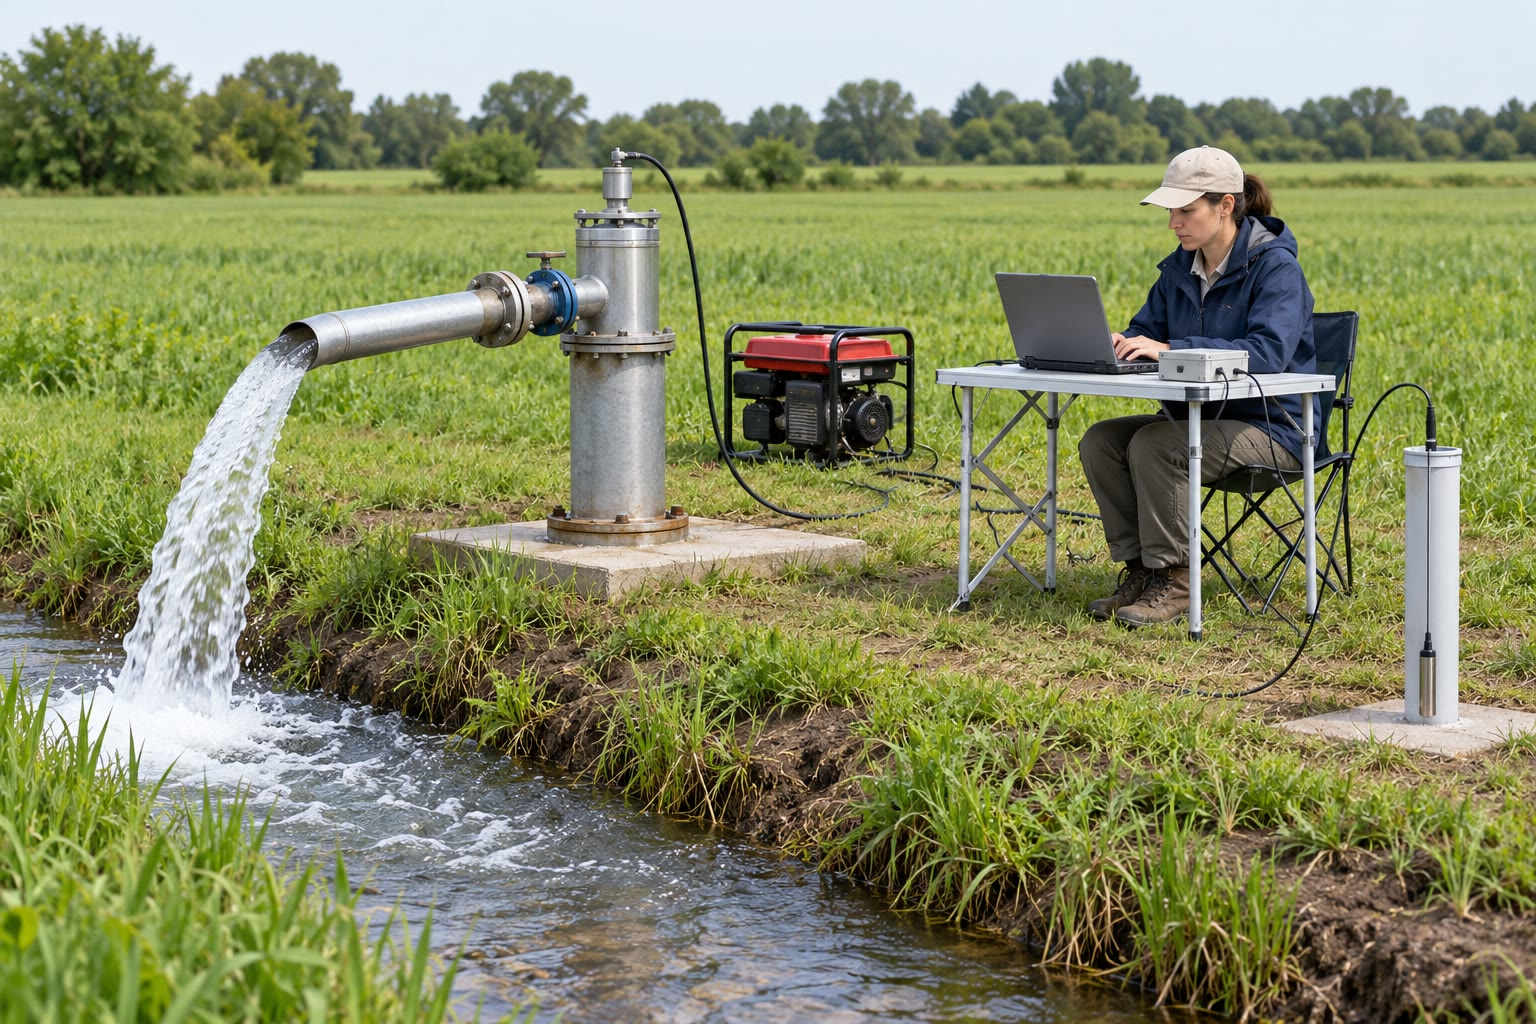
\includegraphics[width=\linewidth]{images/book5/ai/b3-pumping-test.jpg}

{\scriptsize A pumping test: the discharge pipe of the pumped well, a
generator, and a hydrogeologist logging the levels of an observation well
on a laptop (AI-generated illustration).}
\end{minipage}
\end{inthefield}
% ledger: heath:theis, heath:jacob, heath:water-levels, usgs:transducers

\section{Solute transport}\label{sec:b3:hydrogeology:transport}

A solute dissolved in groundwater is carried with the water, at the
\omterm{def:b3:hydrogeology:seepage}{seepage velocity}, and it spreads as it goes: the water in neighbouring
pores moves at different speeds and along different paths, and the solute
also diffuses.

\begin{definition}[Hydrodynamic dispersion; dispersivity]\label{def:b3:hydrogeology:ade}
\emph{Hydrodynamic dispersion}\index{hydrodynamic dispersion} is the
spreading of a solute in flowing groundwater by the variations of the
velocity of the water from pore to pore and by molecular diffusion. Along
the flow it is described by a dispersion coefficient $D = \alpha_Lv + D^*$,
$v$ the \omterm{def:b3:hydrogeology:seepage}{seepage velocity}, $D^*$ the effective molecular diffusivity, and
$\alpha_L$, a length, the longitudinal
\emph{dispersivity}\index{dispersivity} of the medium.
\end{definition}

\begin{theorem}[Advection--dispersion equation]\label{thm:b3:hydrogeology:ade}
Along a one-dimensional flow of constant \omterm{def:b3:hydrogeology:seepage}{seepage velocity} $v$, the
concentration $C(x, t)$ of a non-reacting solute obeys
\[
\frac{\partial C}{\partial t} = D\,\frac{\partial^2C}{\partial x^2} -
v\,\frac{\partial C}{\partial x} .
\]
If the concentration is held at $C_0$ at $x = 0$ from $t = 0$, in a medium
initially free of solute,
\[
\frac{C}{C_0} = \frac12\left[\operatorname{erfc}\frac{x - vt}{2\sqrt{Dt}} +
\mathrm e^{vx/D}\operatorname{erfc}\frac{x + vt}{2\sqrt{Dt}}\right] .
\]
\end{theorem}
\index{advection--dispersion equation}

\begin{proof}
In a slice of unit cross-section and length $\mathrm dx$, of effective
porosity $n_e$, the solute stored is $n_eC\,\mathrm dx$. Its flux is
$n_e(vC - D\,\partial C/\partial x)$, carried with the water and spread by
dispersion as Fick's law spreads a diffusing substance. Conservation gives
$n_e\partial_tC = -\partial_x[n_e(vC - D\partial_xC)]$, the equation. That
the formula satisfies it and the conditions is admitted here;
\cref{exo:b3:hydrogeology:12} checks its spreading.
\end{proof}

In the frame moving with the water, $\xi = x - vt$, the equation is the
diffusion equation, and the front spreads as $\sqrt{2Dt} = \sqrt{2\alpha_L
vt} = \sqrt{2\alpha_Lx}$: the width of the front grows as the square root
of the distance travelled.

\begin{definition}[Retardation factor]\label{def:b3:hydrogeology:retardation}
A solute that is adsorbed on the grains, in equilibrium and in proportion
to its concentration, travels more slowly than the water. Its
\emph{retardation factor}\index{retardation factor (sorption)} is
\[
R = 1 + \frac{\rho_bK_d}{n} ,
\]
$\rho_b$ being the dry bulk density of the medium, $n$ its porosity and
$K_d$ the distribution coefficient, the adsorbed mass per unit mass of
solid divided by the concentration in the water. The solute moves at $v/R$
and disperses with $D/R$.
\end{definition}

\begin{omfigure}
\begin{tikzpicture}
\begin{groupplot}[group style={group size=2 by 1, horizontal sep=1.5cm},
  width=0.48\linewidth, height=0.4\linewidth,
  tick label style={font=\scriptsize}, label style={font=\small}, title style={font=\small}]
\nextgroupplot[xlabel={time (days)}, ylabel={$C/C_0$ at \qty{100}{m}},
  xmin=0, xmax=1000, ymin=0, ymax=1.05, title={breakthrough curves},
  legend style={font=\scriptsize, at={(0.97,0.03)}, anchor=south east}]
% computed in figdata/bachelor-3/advection_dispersion.py
\addplot[omDef, thick] table[x=t, y=c1] {figdata/out/bachelor-3-advection_dispersion-btc.dat};
\addlegendentry{$\alpha_L = \qty{1}{m}$}
\addplot[omMeth, thick] table[x=t, y=c3] {figdata/out/bachelor-3-advection_dispersion-btc.dat};
\addlegendentry{$\alpha_L = \qty{3}{m}$}
\addplot[omThm, thick] table[x=t, y=c10] {figdata/out/bachelor-3-advection_dispersion-btc.dat};
\addlegendentry{$\alpha_L = \qty{10}{m}$}
\addplot[black, thick, densely dashed, forget plot] table[x=t, y=cR] {figdata/out/bachelor-3-advection_dispersion-btc.dat};
\node[font=\scriptsize, anchor=west, align=left] at (axis cs:640,0.45) {$\alpha_L = \qty{3}{m}$,\\ $R = 3$};
\addplot[black!40, densely dotted, forget plot] coordinates {(200,0) (200,1.05)};
\nextgroupplot[xlabel={distance (\unit{m})}, ylabel={$C/C_0$ after 150 days},
  xmin=0, xmax=160, ymin=0, ymax=1.05, title={profiles},
  legend style={font=\scriptsize, at={(0.03,0.03)}, anchor=south west}]
\addplot[omDef, thick] table[x=x, y=c1] {figdata/out/bachelor-3-advection_dispersion-profile.dat};
\addlegendentry{$\alpha_L = \qty{1}{m}$}
\addplot[omMeth, thick] table[x=x, y=c3] {figdata/out/bachelor-3-advection_dispersion-profile.dat};
\addlegendentry{$\alpha_L = \qty{3}{m}$}
\addplot[omThm, thick] table[x=x, y=c10] {figdata/out/bachelor-3-advection_dispersion-profile.dat};
\addlegendentry{$\alpha_L = \qty{10}{m}$}
\addplot[black!40, densely dotted, forget plot] coordinates {(75,0) (75,1.05)};
\end{groupplot}
\end{tikzpicture}

\par\smallskip{\small A solute injected continuously at $x = 0$ into a
flow of \omterm{def:b3:hydrogeology:seepage}{seepage velocity} \qty{0.5}{m/d}. Left, the concentration
\qty{100}{m} down-gradient against time: the water itself arrives after
200 days (dotted); the larger the \omterm{def:b3:hydrogeology:ade}{dispersivity}, the earlier the first
traces and the later the full concentration. An adsorbed solute with $R =
3$ arrives three times later. Right, the concentration along the flow after
150 days, when the water has travelled \qty{75}{m}
(dotted).}\label{fig:b3:hydrogeology:transport}
\end{omfigure}

Dispersivities are hard to measure, and in practice they are often set by
rules of thumb. The oldest takes the longitudinal \omterm{def:b3:hydrogeology:ade}{dispersivity} as a tenth of
the length of the plume. A compilation of field measurements published in
1992 shows that the \omterm{def:b3:hydrogeology:ade}{dispersivity} grows with the scale of the experiment,
that reliable values at large scales are few, and that at any one scale the
values spread over two or three orders of magnitude.
% ledger: epa:dispersivity

\section{Exercises}

\begin{exercise}[$\star$]\label{exo:b3:hydrogeology:1}
Two piezometers stand side by side on ground at \qty{120.0}{m} above the
datum. The first is screened at \qty{40}{m} depth and its water stands
\qty{12.5}{m} below the ground; the second is screened at \qty{80}{m}
depth, its water \qty{15.0}{m} below the ground. Compute the elevation
head, pressure head and \omterm{def:b3:hydrogeology:head}{hydraulic head} at both screens. Which way does the
water flow between them, and under what vertical gradient?
\end{exercise}

\begin{exercise}[$\star$]\label{exo:b3:hydrogeology:2}
A column of sand \qty{50}{cm} long and \qty{10}{cm} in diameter, with $K =
\qty{12}{m/d}$ and an effective porosity of 0.35, carries water under a
head difference of \qty{30}{cm}. Compute the \omterm{def:b3:hydrogeology:darcy}{specific discharge}, the flow
in litres per hour, and the \omterm{def:b3:hydrogeology:seepage}{seepage velocity}.
\end{exercise}

\begin{exercise}[$\star$]\label{exo:b3:hydrogeology:3}
A limestone has $K = \qty{2.5}{m/d}$ for water at \qty{10}{\celsius}
($\rho = \qty{999.7}{kg/m^3}$, $\mu = \qty{1.306e-3}{Pa.s}$). Compute its
\omterm{def:b3:hydrogeology:darcy}{intrinsic permeability}, and its \omterm{def:b3:hydrogeology:darcy}{hydraulic conductivity} for water at
\qty{20}{\celsius} ($\rho = \qty{998.2}{kg/m^3}$, $\mu =
\qty{1.002e-3}{Pa.s}$).
\end{exercise}
% ledger: nist:water

\begin{exercise}[$\star$]\label{exo:b3:hydrogeology:4}
The confined limestone of Varden-3 is \qty{180}{m} thick, with $K =
\qty{2.5}{m/d}$. Compute its \omterm{def:b3:hydrogeology:storage}{transmissivity}, and the \omterm{def:b3:hydrogeology:storage}{storativity} it would
have if only the expansion of the water, \num{9e-7} per metre of aquifer
per metre of head, released water. Compare with $S = \num{2e-4}$.
\end{exercise}
% ledger: heath:storage

\begin{exercise}[$\star\star$]\label{exo:b3:hydrogeology:5}
After a long period of pumping at \qty{1500}{m^3/d}, the drawdowns have
stopped changing: \qty{2.35}{m} in an observation well \qty{20}{m} from the
pumped well and \qty{0.82}{m} in one \qty{200}{m} away. The aquifer is
confined and \qty{40}{m} thick. Compute its \omterm{def:b3:hydrogeology:storage}{transmissivity} and \omterm{def:b3:hydrogeology:darcy}{hydraulic
conductivity}.
\end{exercise}

\begin{exercise}[$\star\star$]\label{exo:b3:hydrogeology:6}
A well pumps \qty{1200}{m^3/d} from a \omterm{def:b3:hydrogeology:aquifer-types}{confined aquifer} with $T =
\qty{300}{m^2/d}$ and $S = \num{5e-4}$. Compute $u$, $W(u)$ (from the
series) and the drawdown \qty{300}{m} away after 1 day and after 10 days.
\end{exercise}

\begin{exercise}[$\star\star$]\label{exo:b3:hydrogeology:7}
For the Varden-3 test ($T = \qty{450}{m^2/d}$, $S = \num{2e-4}$), after
how many minutes may the Cooper--Jacob line be used in observation wells
\qty{60}{m} and \qty{500}{m} from the pumped well? What does this say
about where the observation wells of a short test should be?
\end{exercise}

\begin{exercise}[$\star\star$]\label{exo:b3:hydrogeology:8}
Two wells \qty{400}{m} apart in the Varden limestone each pump
\qty{2160}{m^3/d}. Compute the drawdown after 10 days midway between them,
and at the second well's site due to the first well alone. Why does the
pumping of each well cost the other money?
\end{exercise}

\begin{exercise}[$\star\star$]\label{exo:b3:hydrogeology:9}
In the \omterm{def:b3:hydrogeology:flow-net}{flow net} under the dam, count the flow channels and the head drops.
With $K = \qty{5}{m/d}$ and $H = \qty{10}{m}$, compute the seepage per
metre of dam and under a dam \qty{300}{m} long.
\end{exercise}

\begin{exercise}[$\star\star\star$]\label{exo:b3:hydrogeology:10}
Model a clean sand as straight tubes of radius \qty{50}{\micro\metre} with a
porosity of 0.30. Compute $k$ and $K$ (for water at \qty{20}{\celsius}, as in
\cref{exo:b3:hydrogeology:3}),
and compare with the range for clean sand. Which features of a real sand
does the model leave out, and in which direction does each move $K$?
\end{exercise}
% ledger: nist:water, heath:k-chart

\begin{exercise}[$\star\star\star$]\label{exo:b3:hydrogeology:11}
(a)~Show that the Cooper--Jacob drawdown vanishes at $r_0 =
\sqrt{2.25\,Tt/S}$. (b)~Compute $r_0$ after 30 days of pumping in the
confined Varden limestone, and for the same rock unconfined, with $S =
0.2$. (c)~Why can the cone of a \omterm{def:b3:hydrogeology:aquifer-types}{confined aquifer} reach a boundary that the
test was not meant to see?
\end{exercise}
% ledger: heath:jacob, heath:storage

\begin{exercise}[$\star\star\star$]\label{exo:b3:hydrogeology:12}
(a)~For a long travel distance the breakthrough curve at $x$ is close to a
normal distribution in time, of mean $x/v$ and standard deviation $\sigma_t
= \sqrt{2\alpha_Lx}/v$. Show it from the spreading $\sqrt{2Dt}$ of the front.
(b)~At \qty{100}{m}, with $v = \qty{0.5}{m/d}$, the concentration reaches
\qty{16}{\percent} after \num{152.6}~days and \qty{84}{\percent} after
\num{247.2}~days. Estimate $\alpha_L$. (c)~A sandy aquifer has $\rho_b =
\qty{1.9}{g/cm^3}$ and $n = 0.30$; a solute has $K_d =
\qty{0.32}{cm^3/g}$. Compute $R$.
\end{exercise}

\section{Problem: Pumping Test at Varden-3}

\begin{problem}[{Weekend problem --- heads, a pumping test and the travel of
a pollutant in the confined limestone of the Varden Hills}]
\label{pb:b3:hydrogeology:1}
The invented well Varden-3 is drilled at (4500, 5000) on the grid of the
Varden Hills, from a ground elevation of \qty{363.2}{m}, through the
Jurassic shale into the Jurassic limestone, whose top lies at
\qty{282.5}{m} and base at \qty{102.5}{m} above sea level; the well is open
over the full thickness of the limestone. Before the test the water in it
stands \qty{45.0}{m} below the ground.

\medskip\noindent\textbf{Part I --- The aquifer and its natural flow.}
\begin{enumerate}
\item Compute the thickness of the shale and of the limestone at the well.
\item Compute the head in the limestone and the pressure head at its top.
  Why is the limestone a \omterm{def:b3:hydrogeology:aquifer-types}{confined aquifer} here?
\item Three piezometers open to the limestone stand at P1 (4300, 5250), P2
  (4850, 5150) and P3 (4550, 4650), with heads of 318.96, 317.34 and
  \qty{317.52}{m}. Writing $h = ax + by + c$, find $a$ and $b$.
\item Compute the \omterm{def:b3:hydrogeology:head}{hydraulic gradient} and the azimuth towards which the
  water flows.
\end{enumerate}

\medskip\noindent\textbf{Part II --- The pumping test.} The well is pumped
at \qty{2160}{m^3/d} for two days. In an observation well \qty{60}{m}
away the drawdowns are:
\begin{center}
\begin{tabular}{l*{11}{c}}
\hline
$t$ (\unit{min}) & 1 & 2 & 3 & 5 & 7 & 10 & 15 & 20 & 30 & 45 & 60\\
$s$ (\unit{m}) & 0.18 & 0.36 & 0.48 & 0.64 & 0.77 & 0.88 & 1.04 & 1.15 & 1.30 & 1.45 & 1.56\\
\hline
$t$ (\unit{min}) & 90 & 120 & 180 & 240 & 360 & 480 & 720 & 960 & 1440 & 2160 & 2880\\
$s$ (\unit{m}) & 1.71 & 1.82 & 1.98 & 2.08 & 2.24 & 2.35 & 2.50 & 2.61 & 2.77 & 2.92 & 3.03\\
\hline
\end{tabular}
\end{center}
\begin{enumerate}[resume]
\item Plot $s$ against $\log_{10}t$. Which early points leave the straight
  line, and why?
\item From the straight part, measure the drawdown per log cycle.
\item Compute the \omterm{def:b3:hydrogeology:storage}{transmissivity}.
\item Find the time $t_0$ at which the line meets zero drawdown.
\item Compute the \omterm{def:b3:hydrogeology:storage}{storativity}.
\item Check that $u \le 0.05$ for the points you used.
\item Compute the \omterm{def:b3:hydrogeology:darcy}{hydraulic conductivity} of the limestone.
\end{enumerate}

\medskip\noindent\textbf{Part III --- The cone.} From here take $T =
\qty{450}{m^2/d}$ and $S = \num{2e-4}$.
\begin{enumerate}[resume]
\item Compute the Theis drawdown in the observation well after 2 days and
  compare with the record.
\item A farm well \qty{1}{km} away draws on the same limestone. Compute its
  drawdown after 30 days of pumping.
\item Compute Jacob's distance $r_0$ after 30 days. What does it say about
  the edges of the aquifer and the fault of the Varden Hills?
\item Compute the volume pumped in 30 days. Where, in a \omterm{def:b3:hydrogeology:aquifer-types}{confined aquifer},
  does it come from?
\item How would the drawdown at the farm compare if the limestone were
  unconfined, with $S = 0.18$?
\end{enumerate}

\medskip\noindent\textbf{Part IV --- A pollutant.} A leak of a dissolved
pollutant reaches the limestone \qty{200}{m} from the well. Take an
effective porosity of 0.18 and a \omterm{def:b3:hydrogeology:retardation}{retardation factor} of 2.5.
\begin{enumerate}[resume]
\item Before the pumping, compute the \omterm{def:b3:hydrogeology:darcy}{specific discharge} and the \omterm{def:b3:hydrogeology:seepage}{seepage
  velocity} of the natural flow of Part~I.
\item How long would the water take to cover \qty{200}{m}, and the
  pollutant?
\item With the well pumping, and the leak up-gradient of it, the flow
  becomes radial towards the well. Show that the water takes $t = \pi n_e b
  r^2/Q$ to reach the well from a distance $r$, neglecting the natural
  flow, and compute it for the water and for the pollutant.
\item With the rule of thumb of a \omterm{def:b3:hydrogeology:ade}{dispersivity} a tenth of the distance,
  estimate the spreading $\sqrt{2\alpha_Lx}$ of the front at the well. What
  does it mean for the first arrival?
\item Should the pumping go on? Give one argument for and one against.
\item Give the \omterm{def:b3:hydrogeology:storage}{transmissivity} of the Varden limestone aquifer, in square
  metres per day, to two significant figures.
\end{enumerate}
\end{problem}
% ledger: heath:jacob, heath:theis, heath:storage, epa:dispersivity, region:name
